%results & evaluation, explicitly mentioning of known limitations

We are able to fully generate terrains, including elevations, biomes and rivers.
Figure~\ref{fig:generator} shows a generated map. It is also possible to export this generated map with all associated data.

\begin{figure}[H]
	\centering
	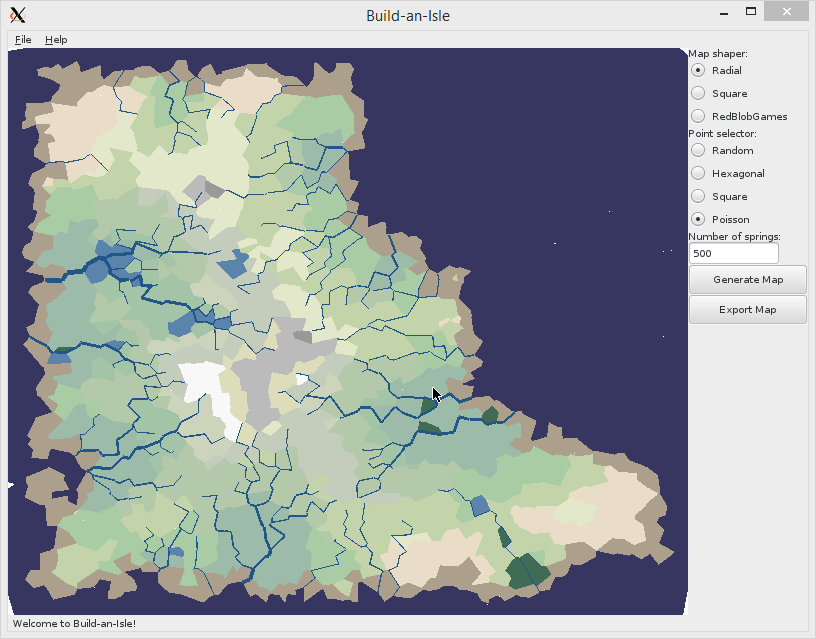
\includegraphics[width=0.8\linewidth]{topdown}
	\caption{A generated map}
	\label{fig:generator}
\end{figure}

\begin{figure}[H]
	\centering
	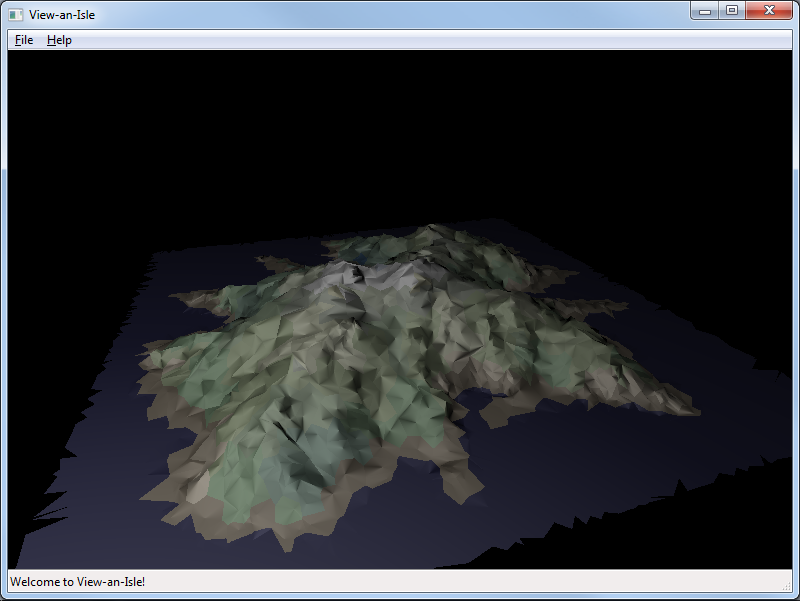
\includegraphics[width=0.8\linewidth]{resultsmallnorivers}
	\caption{A small map without rivers for which geometry has been generated}
	\label{fig:resultsmall}
\end{figure}

\begin{figure}[H]
	\centering
	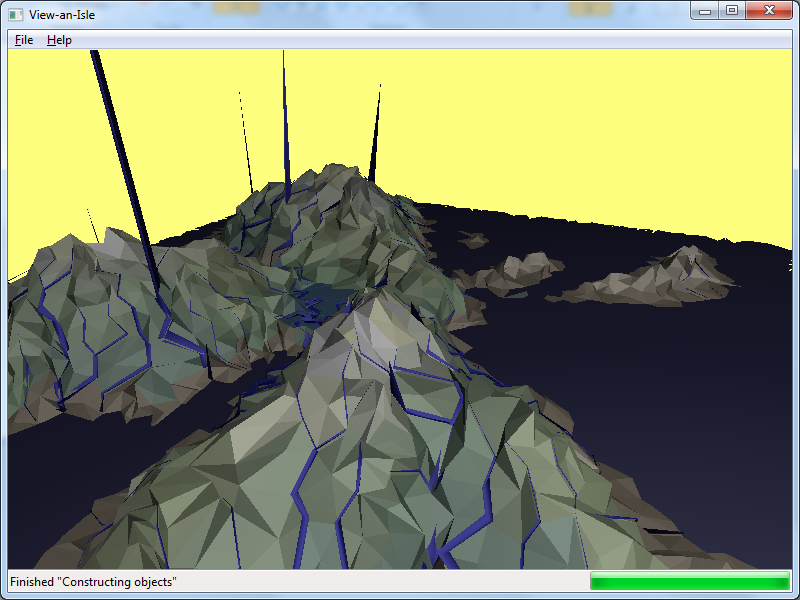
\includegraphics[width=0.8\linewidth]{shamefulldisplay}
	\caption{There are cases where rivers can be visualised without standing out, however many of the generated maps will contain small polygons that lead to unpredictable geometric river representations. It would take a significant amount of time to improve the current method.}
	\label{fig:resultsriver}
\end{figure}

\begin{figure}[H]
	\centering
	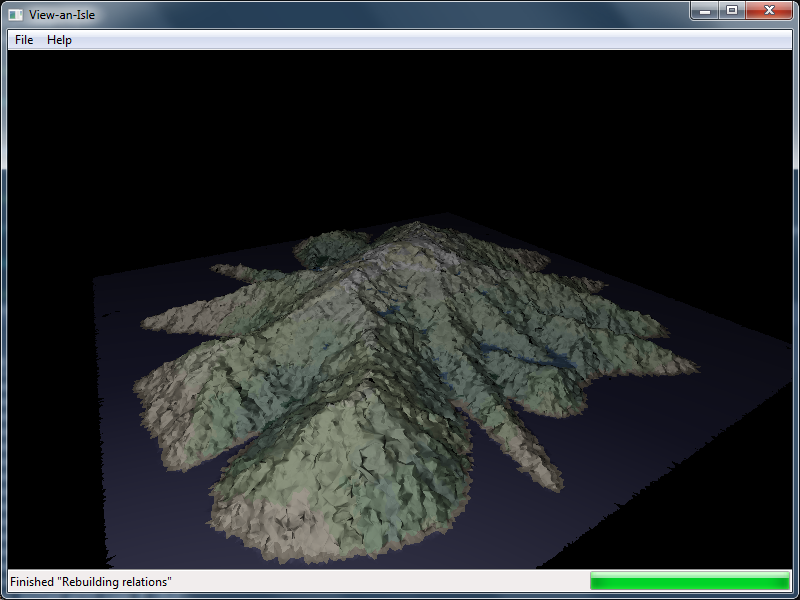
\includegraphics[width=0.8\linewidth]{resultlargenorivers}
	\caption{A large map showcasing a body of water situated high above sea level}
	\label{fig:resultslarge}
\end{figure}

The plans for the viewer were more extensive than what we were able to achieve. We encountered several unforseen problems which did turn out to be solvable but this obviously took a significant amount of time. The viewer is able to import map files created by the generator and construct appropriate geometry. It is also able to take the borders that are indicated to have rivers running along them and define geometric representation for these rivers. Figure~\ref{fig:resultsriver} shows that this is far from perfect, however the generator could be limited to generating more regular voronoi diagrams to avoid these situations. In the end we were able to produce satisfying visualisations of randomly generated maps as shown in Figure~\ref{fig:resultslarge}.